\subsection{Results for $y$ Offset}
%\label{subsec:latitude_no_abs_results}
%\vspace{10pt}

Figure~\ref{fig:var_lat} represents the $p$-values for the Wilcoxon signed-rank test on actual and predicted values across $k$-fold validation datasets for the $y$ offset in the $k$-fold testing datasets using different RNN models, and forecasting times. Darker colors in grayscale represent a higher $p$-value in a range from $0$ to $1$. The values on the secondary diagonal are all equal to $1$ and black because models equal themselves.

\begin{figure}[!ht]
	\centering
	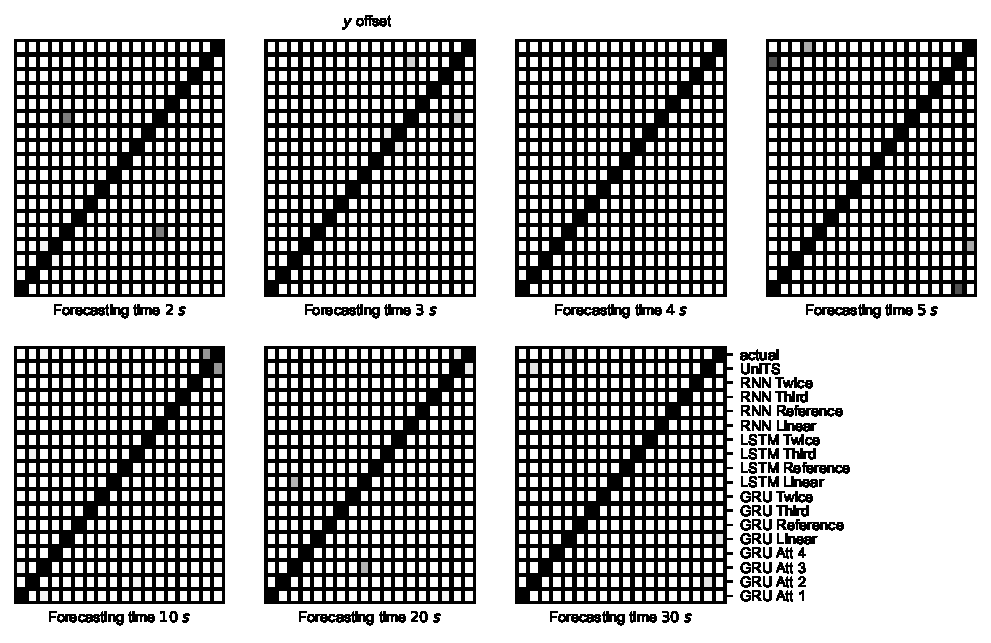
\includegraphics[width = 0.99 \linewidth]{var_lat.pdf}
	\caption{The $p$-values for the Wilcoxon signed-rank test on actual and predicted values across $k$-fold validation datasets for the $y$ offset in the $k$-fold testing datasets using different RNN models, and forecasting times. Darker colors in grayscale represent a higher $p$-value in a range from $0$ to $1$. The values on the secondary diagonal are all equal to $1$ and black because models equal themselves.}
	\label{fig:var_lat}
\end{figure}

The average RMSE ($\times 10^{-4}$), with standard deviation in brackets, across $k$-fold validation datasets for the $y$ offset estimated on the $k$-fold testing datasets by different RNN models, and forecasting times is listed in Table~\ref{tab:best_latitude_no_abs_RMSE}.

\begin{table}[!ht]
	\centering
	\resizebox{\linewidth}{!}{
		\begin{tabular}{|c|c|c|c|c|c|c|c|}
			\hline
			Model & $2$ $s$ & $3$ $s$ & $4$ $s$ & $5$ $s$ & $10$ $s$ & $20$ $s$ & $30$ $s$ \\ \hline
			\multirow{2}{*}{GRU Att 2} & $1.302$ & $1.584$ & $\mathbf{1.76}$ & $\mathbf{2.007}$ & $3.125$ & $4.289$ & $5.054$ \\
			 & ($0.207$) & ($0.238$) & \textbf{(}$\mathbf{0.198}$\textbf{)} & \textbf{(}$\mathbf{0.213}$\textbf{)} & ($0.26$) & ($0.325$) & ($0.438$) \\ \hline
			\multirow{2}{*}{GRU Reference} & $\mathbf{1.027}$ & $1.757$ & $2.219$ & $2.533$ & $3.711$ & $5.019$ & $5.615$ \\
			 & \textbf{(}$\mathbf{0.266}$\textbf{)} & ($0.357$) & ($0.352$) & ($0.251$) & ($0.276$) & ($0.34$) & ($0.395$) \\ \hline
			\multirow{2}{*}{LSTM Third} & $1.189$ & $\mathbf{1.473}$ & $2.049$ & $2.383$ & $3.701$ & $5.04$ & $5.616$ \\
			 & ($0.346$) & \textbf{(}$\mathbf{0.36}$\textbf{)} & ($0.479$) & ($0.349$) & ($0.23$) & ($0.386$) & ($0.406$) \\ \hline
			\multirow{2}{*}{UniTS} & $1.343$ & $1.586$ & $1.811$ & $2.017$ & $\mathbf{2.831}$ & $\mathbf{3.821}$ & $\mathbf{4.357}$ \\
			 & ($0.248$) & ($0.217$) & ($0.21$) & ($0.21$) & \textbf{(}$\mathbf{0.238}$\textbf{)} & \textbf{(}$\mathbf{0.301}$\textbf{)} & \textbf{(}$\mathbf{0.331}$\textbf{)} \\ \hline
		\end{tabular}
	}
	\caption{The average RMSE ($\times 10^{-4}$), with standard deviation in brackets, across $k$-fold validation datasets for the $y$ offset estimated on the $k$-fold testing datasets by different RNN models, and forecasting times.}
	\label{tab:best_latitude_no_abs_RMSE}
\end{table}

The GRU Att 2 model achieved the lowest RMSE for $y$ offset, and a forecasting time of $4$, and $5$ $s$ with average values and standard deviation (in brackets) that equal $17.603 \times 10^{-5}$ $\degree$ ($1.979 \times 10^{-5}$ $\degree$), and $20.067 \times 10^{-5}$ $\degree$ ($2.131 \times 10^{-5}$ $\degree$) respectively.

The GRU Att 2 model does not have a statistically significantly different RMSE than the GRU Att 1, LSTM Third, LSTM Twice, and UniTS models for $y$ offset using a forecasting time of $4$ $s$, with $p$-values equaling $2.551 \times 10^{-2}$, $4.605 \times 10^{-3}$, $1.453 \times 10^{-3}$, and $6.129 \times 10^{-3}$.

\markertable{tab:\label{tab:RMSE:latitude:no:abs:p:4}}

The GRU Att 2 model does not have a statistically significantly different RMSE than the GRU Att 1, and UniTS models for $y$ offset using a forecasting time of $5$ $s$, with $p$-values equaling $1.355 \times 10^{-2}$, and $3.525 \times 10^{-1}$.

\markertable{tab:\label{tab:RMSE:latitude:no:abs:p:5}}

The GRU Reference model achieved the lowest RMSE for $y$ offset, and a forecasting time of $2$ $s$ with an average value and standard deviation (in brackets) that equals $10.265 \times 10^{-5}$ $\degree$ ($2.66 \times 10^{-5}$ $\degree$).

The GRU Reference model does not have a statistically significantly different RMSE than the GRU Att 1, GRU Linear, GRU Third, GRU Twice, LSTM Linear, LSTM Reference, and LSTM Third models for $y$ offset using a forecasting time of $2$ $s$, with $p$-values equaling $3.781 \times 10^{-3}$, $1.908 \times 10^{-1}$, $9.573 \times 10^{-2}$, $6.338 \times 10^{-1}$, $3.419 \times 10^{-3}$, $1.485 \times 10^{-1}$, and $9.032 \times 10^{-2}$.

\markertable{tab:\label{tab:RMSE:latitude:no:abs:p:2}}

The LSTM Third model achieved the lowest RMSE for $y$ offset, and a forecasting time of $3$ $s$ with an average value and standard deviation (in brackets) that equals $14.733 \times 10^{-5}$ $\degree$ ($3.604 \times 10^{-5}$ $\degree$).

The LSTM Third model does not have a statistically significantly different RMSE than the GRU Att 1, GRU Att 2, GRU Att 3, GRU Att 4, GRU Linear, GRU Reference, GRU Third, GRU Twice, LSTM Linear, LSTM Reference, and UniTS models for $y$ offset using a forecasting time of $3$ $s$, with $p$-values equaling $1.874 \times 10^{-2}$, $2.748 \times 10^{-2}$, $4.895 \times 10^{-4}$, $3.088 \times 10^{-3}$, $5.072 \times 10^{-3}$, $1.027 \times 10^{-3}$, $9.032 \times 10^{-2}$, $6.721 \times 10^{-1}$, $2.191 \times 10^{-2}$, $4.605 \times 10^{-3}$, and $8.822 \times 10^{-3}$.

\markertable{tab:\label{tab:RMSE:latitude:no:abs:p:3}}

The UniTS model achieved the lowest RMSE for $y$ offset, and a forecasting time of $10$, $20$, and $30$ $s$ with average values and standard deviation (in brackets) that equal $28.309 \times 10^{-5}$ $\degree$ ($2.382 \times 10^{-5}$ $\degree$), $38.21 \times 10^{-5}$ $\degree$ ($3.005 \times 10^{-5}$ $\degree$), and $43.569 \times 10^{-5}$ $\degree$ ($3.311 \times 10^{-5}$ $\degree$) respectively.

